\documentclass[12pt]{article}

\usepackage{fancyhdr}
\usepackage{geometry}
\usepackage{ucs}
\usepackage[utf8x]{inputenc}
\usepackage[T1]{fontenc}
\usepackage[ngerman]{babel}
\usepackage{amsmath,amssymb,amstext}
\usepackage{hyperref}
\usepackage{cancel}
\usepackage{dsfont}
\usepackage{physics}
\usepackage{lmodern}
\usepackage{enumerate}
\usepackage{enumitem}
\usepackage{graphicx}
\usepackage{listings, color}
\usepackage[labelfont=bf]{caption}
\usepackage{titling}

\lstset{basicstyle=\scriptsize} %Quellcode mit Umlauten und ganz klein
\lstset{literate=
  {Ö}{{\"O}}1
  {Ä}{{\"A}}1
  {Ü}{{\"U}}1
  {ß}{{\ss}}2
  {ü}{{\"u}}1
  {ä}{{\"a}}1
  {ö}{{\"o}}1
}


%Geometrie----------------------------------------------------------------------------------------------------------

\geometry{a4paper, top=25mm, left=15mm, right=15mm, bottom=25mm,headsep=10mm, footskip=10mm}
\pagestyle{fancy}
\setlength{\parindent}{0pt} %Zeileneinrückung

\fancyhf{} %Setzt voreingestellte Kopf-und Fußzeilen-Eigenschaften zurück

\lhead{\nouppercase{\leftmark}}
\chead{}
\rhead{\thepage}

\lfoot{}
\cfoot{}
\rfoot{}

\title{\vspace{0cm}{\Huge Fortgeschrittenen-Praktikum I:\\ \vspace{1cm} Ultraschall}}
\author{Saskia Bondza\\Simon Stephan}
\date{durchgeführt am 20./21.09.2016}

\pretitle{%
  \begin{center}
  \LARGE
  
\includegraphics[width=6cm,]{figures/siegel}\\[\bigskipamount]
}
\posttitle{\end{center}}

%neue Commands----------------------------------------------------------------------------------------------------------
\newcommand{\nab}{\vec{\nabla}} %direkter Befehl mit Vektorpfeil
\newcommand{\gra}[3][0.7]{
	\begin{minipage}[h!]{\textwidth}
		\centering
		\includegraphics[width=#1\textwidth]{figures/#2.png}
		\captionof{figure}{#3}
	\end{minipage}
	\vskip 30 pt
}
\newcommand{\graTwo}[4][0.5]{
	\begin{minipage}[h!]{\textwidth}
		\centering
		\includegraphics[width=#1\textwidth]{figures/#2.png}
		\includegraphics[width=#1\textwidth]{figures/#3.png}
		\captionof{figure}{#4}
	\end{minipage}
	\vskip 30 pt
}
\newcommand{\del}[2][]{\frac{\partial #1}{\partial #2}}
\newcommand{\code}[1]{\texttt{#1}}


%Titel,Inhalt----------------------------------------------------------------------------------------------------------

\begin{document}
\pagenumbering{gobble} %verstecke Seitenzahl
\maketitle
\newpage

\thispagestyle{empty}
\section*{Abstract}


In diesem Versuch wird über die Messung von Beugungs-Spektren eines He-Ne-Lasers ($\lambda = 632,8nm$) die Gitterkonstante verschiedener Gitter (Sinusgitter, Amplitudengitter) und die Aperturfunktion eines bestimmten Gitters bestimmt. Der Hauptteil des Versuches beschäftigt sich mit der Untersuchung von Ultraschallwellen in Flüssigkeit als Phasengitter. Dazu wird die Intensitätsänderung der Beugungsordnung in Abhängigkeit der Spannung des Schallerzeugers (Piezoquarz) ausgewertet, die Wellenlänge der Ultraschallwelle bestimmt Nennerund mit der Raman-Nath-Theorie verglichen.

\newpage
\tableofcontents
\newpage

%Schreiben----------------------------------------------------------------------------------------------------------
\pagenumbering{arabic} %verstecke Seitenzahl
\section{Einleitung}



\newpage
\section{Theoretische Grundlagen}

\subsection{Beugung}

Trifft eine Lichtwelle auf ein Hindernis z.B. einen Spalt wird das Phänomen der Beugung beobachtet. In Abbildung \ref{Fraunhofer} ist  der Grundaufbau eines Experiments zum Nachweis von Beugungsphänomenen (Fraunhofersche Anordnung) dargestellt, der in diesem Experiment verwendet wird. 

\gra{Fraunhofer}{Fraunhofersche Anordnung \label{Fraunhofer}}           

\subsection{Raman-Nath-Theorie}
\label{Raman-Nath}
\newpage
\section{Sinusgitter}

\newpage
\subsection{Versuchsaufbau und -Durchführung}





\newpage
\subsection{Auswertung}

Aus den gemessenen Koordinaten der Punkte $P(x/y)$ der Maxima (siehe \ref{Laborheft})berechnen wir zunächst die Abstände $l_1 = \sqrt{x_1²+y_1²}$ und $l_2= \sqrt{x_2²+y_2²} $ zwischen dem Maximum $0.$ Ordnung und den Maxima $1.$ Ordnung. Aus den beiden Abständen zum linken und rechten Maximum $1.$ Ordnung berechnen wir einen gemittelten Abstand $l_{ges}$. Die Fehler berechnen wir mit Gauß'scher Fehlerfortpflanzung aus dem Fehler $s_{x/y}$ auf die Koordinaten:

\begin{align*}
s_{l_1} = s_{l_2} &= \sqrt{\left(\del[l]{x}\cdot s_{x/y}\right)^2+\left(\del[l]{y}\cdot s_{x/y}\right)^2}\\
&= s_{x/y}\\
\  \\
s_{l_{ges}} &= s_{x/y}/\sqrt{2}
\end{align*}

Wir erhalten:

 \vskip 10 pt
 \begin{table}[h!]
 {\centering{}
\begin{tabular}{c||c|c|c}
 					& $l_1$/cm 	& $l_2$/cm & $l{ges}$/cm	\\ \hline\hline
Messung 1		& $3.9 \pm 0.1$ 	&  $3.9 \pm 0.1$    	&  $3.95 \pm 0.07$ \\ \hline 
Messung 2	&	 $1.9 \pm 0.1$ 	   	&  $1.8 \pm 0.1$  	&  $1.87 \pm 0.07$  \\ \hline
Messung 3      	&  $5.0 \pm 0.1$  	&  $4.9 \pm 0.1$  &  $5.00 \pm 0.07$  \\ \hline
Messung 4    & $2.8 \pm 0.1$ & $2.9 \pm 0.1$ &   $2.88 \pm 0.07$        \\ \hline                                           
Messung 5  & $5.6 \pm 0.1$  & $5.7 \pm 0.1$ & $5.61 \pm 0.07$
 \end{tabular}}
 \caption{Abstände der Beugungsmaxima}
\end{table}
\vskip 10 pt

Hieraus lässt sich nun mit ref!!!!!! die Gitterkonstante berechnen wobei sich der Fehler wieder mit Gauß'scher Fehlerfortpflanzung berechnen lässt:

\begin{align*}
s_g = \sqrt{\left(\del[g]{l}\cdot s_{l}\right)^2+\left(\del[g]{d}\cdot s_{d}\right)^2}
\end{align*}

Wir erhalten:

\begin{itemize}
\item Messung 1: $g = 996 \pm 16$ nm
\item Messung 2: $g = 1082 \pm 40$ nm
\item Messung 3: $g = 989 \pm 13$ nm
\item Messung 4: $g = 994 \pm 23$ nm
\item Messung 5: $g = 995 \pm 12$ nm
\end{itemize}

Als Endergebnis berechnen wir nun noch das gewichtete Mittel mit Fehler:

\begin{align*}
g_{ges} &=\frac{\sum\limits_i \frac{1}{\sigma_i²} \cdot g_i}{\sum\limits_i \frac{1}{\sigma_i²}}\\
s_{g_{ges}} &= \frac{1}{\sum\limits_i \frac{1}{\sigma_i²}}
\end{align*}

und erhalten:

\begin{align*}
g_{ges} = 996 \pm 7 nm
\end{align*}

\newpage
\subsection{Diskussion}

\newpage
\section{Amplitudengitter}

\newpage
\subsection{Versuchsaufbau und -Durchführung}





\newpage
\subsection{Auswertung}

\subsubsection{Referenzgitter}

\label{Happyisttoll}

Da das Oszilloskop eine Zeitdifferenz zwischen den Maxima angibt und keine Winkel, wird mit einem Referenzgitter mit bekannter Gitterkonstante zunächst eine Eichung des Winkel-Zeit-Verhältnisses durchgeführt und ein Umrechnungsfaktor bestimmt. Wir tragen hierfür die Zeit über die theoretische Lage der Maxima auf, die sich aus \[\sin\theta=\frac{n\lambda}{K_R}\] mit $K_R = 0.125 mm$ ergibt und führen einen linearen Fit durch.

\vskip 10 pt
 \begin{table}[h!]
 {\centering{}
\begin{tabular}{c||c|c}
 m & $\sin(\theta)$ & t/$10^{-4}$ \\ \hline\hline
 -2 &$-0.0101$&    $ -1.3427 \pm 0.0011 $  \\ \hline
 -1 &$-0.0051$& $ -0.6719 \pm 0.0005 $     \\ \hline
 0 &$0$&  $ 0\pm 0.0004$         \\ \hline
 1 &$0.0051$&   $ 0.6729 \pm 0.0005 $        \\ \hline
 2 &$0.0101$&     $ 1.3479 \pm 0.0012 $        \\ \hline

 \end{tabular}
 
 \caption{Abstände der Beugungsmaxima}}
\end{table}
\vskip 10 pt

\gra{Zeiteichung}{Zeit-Winkel-Eichung\label{EINHORN}}

Aus der Steigung des Linearen Fits (siehe Abbildung \ref{EINHORN} ) lässt sich nun der Faktor für die Umrechnung von Zeit nach Winkeln bestimmen:

\begin{align*}
a &= (74.35\pm0.05)\,\frac1{\mathrm{s}}&
\text{mit } a = \frac{\sin(\theta))}{t}
\end{align*}

\subsubsection{Bestimmung verschiedener Gitterkonstanten}
Wir haben für 5 verschiedenen unbekannte Amplitudengitter Interferenzmuster aufgenommen und bestimmen nun aus diesen die jeweilige Gitterkonstante. Die Zeitabhängigkeit der Interferenzmuster werden nun mithilfe des in \ref{Happyisttoll} berechneten Wertes in eine $\sin\theta$-Abhängigkeit umgerechnet. Anschließend wird aus den Beugungsordnungen in Abhängigkeit der Positionen der Maxima die Gitterkonstante des jeweiligen Gitters bestimmt. Die Steigung $a$ des linearen Fits $m=\frac{K}{\lambda}\sin\theta$ beträgt nun $a=\frac{K}{\lambda}$. Damit gilt für die Gitterkonstante: $$K=a\cdot\lambda$$.

Wir erhalten nun mit dieser Rechnung die folgenden Werte für die Gitterkonstanten:
\begin{align*}
	K_1&=(129.26\pm0.07)\,\mathrm{\mu m}\\
	K_2&=(34.26\pm0.03)\,\mathrm{\mu m}\\
	K_3&=(102.9\pm0.3)\,\mathrm{\mu m}\\
	K_4&=(72\pm6)\,\mathrm{\mu m}\\
	K_5&=(51.57\pm0.08)\,\mathrm{\mu m}\\
\end{align*}


\subsubsection{Aperturfunktion}


Wir bestimmen die Aperturfunktion für Gitter 1, da wir hier die meisten Maxima beobachten konnten (siehe Abbildung ref!!!).
Aus den Amplituden der gefitteten  Gaußfunktionen erhalten wir hierbei die Intensität, wobei wir wir für jedes Maximum die Amplitude aus linkem und rechtem Maximum gewichtet mitteln (siehe ref!!!). 
 \vskip 10 pt
 \begin{table}[h!]
 {\centering
\begin{tabular}{c||c|c|c}
 					& $I_1/V$ 	& $I_2/V$ & $I_{ges}/V$	\\ \hline\hline
Maximum 5. Ordnung     & $0.08 \pm 0.14$  & $0.040 \pm 0.009$      &  $0.04012 \pm  0.00008$                       \\ \hline
Maximum 4. Ordnung		& $0.186 \pm 0.009$ 	&  $0.177 \pm 0.009$    	&  $0.182 \pm 0.006$ \\ \hline 
Maximum 3. Ordnung	&	 $0.402 \pm 0.009$ 	   	&  $0.447 \pm 0.010$  	&  $0.425 \pm 0.007$  \\ \hline
Maximum 2. Ordnung      	&  $0.95 \pm 0.02$  	&  $0.92 \pm 0.02$  &  $0.935 \pm 0.014$  \\ \hline
Maximum 1. Ordnung    & $2.8 \pm 0.1$ & $2.9 \pm 0.1$ &   $2.88 \pm 0.07$        \\ \hline                                           
Maximumg 0. Ordnung  & -  & - & $2.72 \pm 0.06$
 \end{tabular}
 \caption{Abstände der Beugungsmaxima}}
\end{table}
\vskip 10 pt


Aus diesen und der zuvor berechneten Gitterkonstante $g_1 = (807 \pm 9) nm$ (siehe ref!!!) lässt sich mittels der Fourierreihe (siehe ref!!!) nun die Aperturfunktion näherungsweise bestimmen:

\[f(x)\approx\sum^{5}_{k=0}\pm\sqrt{I_k}\cos\left(\frac{2k\pi x}{g_1} \right) \]

\gra{apertur}{Genäherte Aperturfunktion von Gitter 1} \label{kotz}



Aus der Aperturfunktion bestimmen wir nun die Spaltbreite $b$, indem wir das FHWM durch Bestimmung des Schnittpunktes der Aperturfunktion mit der Konstanten mit dem Wert $x=\frac{max}{2}$  berechnen (siehe Abbildung \ref{LONDOOON}), wobei max für das Maximum der Aperturfunktion steht.

\gra{Spaltbreite}{Bestimmung der Spaltbreite aus der Aperturfunktion}\label{LONDOOON}

Wir erhalten:

\begin{align*}
b = 120 nm
\end{align*}

\newpage
\subsection{Diskussion\label{BOOOOOMMMM!!!!!!!!!}} 

\section{Ultraschall-Phasengitter}

\newpage
\subsection{Versuchsaufbau und -Durchführung}





\newpage
\subsection{Auswertung}
\subsubsection{Zeiteichung}
Wie in \ref{Happyisttoll} haben wir das Referenzgitter mit $K_R=125 \mu m$ zur Zeiteichung benutzt. (siehe Abbildung \ref{simonhatsverkackt})

\graTwo[0.49]{ultraschall-eichgitter}{ultraschall-zeiteichung}{Interferenzmuster des Referenzgitters und linearer Fit zur Bestimmung des Umrechnungsfaktors\label{simonhatsverkackt}}

Aus dem linearen Fit erhalten wir:
\begin{align*}
a &=(70.64\pm0.06)\,\frac1{\mathrm{s}}&
\text{mit } a = \frac{\sin(\theta)}{t}
\end{align*}

\subsubsection{Bestimmung der Beugungsmaxima}
\gra[1]{ultraschall-regenbogen}{Interferenzmuster der Ultraschallwelle für verschiedene Spannungen \label{regenbogen}}
In Abbildung \ref{regenbogen} sind die Beugungsbilder an der Ultraschallwelle für verschiedene Spannungen aufgetragen. An diese Beugungsmuster haben wir eine Summe von Gaußfunktionen gefittet. Die Ergebnisse der Fits sind im Anhang unter \ref{fitergebnisse} zu finden. Bei hohen Spannungen lassen sich bis zu 3 Beugungsordnungen sehen und sinnvoll aus dem Fit bestimmen, wobei bei niedrigen Spannungen nur noch das nullte Hauptmaximum zu bestimmen ist. 

\subsubsection{Berechnung der Intensitäten an den Maxima}
Da nicht für jede Spannung alle Beugungsmaxima zu sehen sind, wurde für jedes Maximum über alle für dieses Maximum bestimmten Positionen gewichtet gemittelt und an den Kurven, an denen diese Beugungsordnung nicht zu erkennen ist, für die Intensität der Funktionswert des Fits an der gemittelten Position benutzt. Nun werden die Intensitäten $I$ mit $\hat{I}=\frac{I}{I_0}$ genormt. $I_0$ ist hierbei die Intensität am Maximum nullter Ordnung bei der Spannung $U=0$V.

\subsubsection{Überprüfung der Raman-Nath-Theorie}
Die Raman-Nath-Theorie (siehe \ref{Raman-Nath}) besagt, dass sich die Intensität in Abhängigkeit der Spannung nach folgender Formel verhält:
\begin{align}
	I_m&=J_m^2(\alpha U) \label{besselquadratfunktion}
\end{align}
$J_m(x)$ sind hierbei die Besselfunktionen.

\gra{ultraschall-besselfits}{Normierte Intensität der Beugungsmaxima über die Spannung mit Besselquadratfits zur Überprüfung der Raman-Nath-Theorie\label{besselfits}}

In Abbildung \ref{besselfits} sieht man die an die Daten gefitteten Funktionen. Tabelle \ref{besselfitdaten} zeigt die Parameter der gefitteten Funktionen.

\begin{table}[h!]
	\centering{
		
		\begin{tabular}{c|c}
			
			m&$\alpha$\\\hline
			-3&$0,271\pm0,005$\\
			-2&$0,225\pm0,003$\\
			-1&$0,271\pm0,012$\\
			 0&$0,164\pm0,004$\\
			 1&$0,271\pm0,012$\\
			 2&$0,243\pm0,004$\\
			 3&$0,280\pm0,003$\\			
		\end{tabular}
		\caption{Fitparameter $\alpha$ der Besselquadratfits (siehe Formel (\ref{besselquadratfunktion}))\label{besselfitdaten}}
		}
\end{table}

\subsubsection{Bestimmung der Wellenlänge von Isooktan}
Aus den Abständen der Beugungsordnungen der Interferenz an der Schallwelle kann nun, analog zu REFERENZ AMPLITUDENGITTER, die Wellenlänge der Schallwelle bestimmt werden: $$m=\frac{\Lambda}{\lambda}\sin\theta$$
In Abbildung \ref{schallwellenlaenge} haben wir durch einen linearen Fit die Steigung $a$ von $m$ über $\sin\theta$ bestimmt. Daraus erhalten wir die Wellenlänge der Schallwelle mit:
$$\Lambda=a\cdot\lambda=(557\pm2) \,\mathrm{\mu m}$$
\gra{schallwellenlaenge}{Bestimmung der Schallwellenlänge aus der Steigung von $m$ über $\sin\theta$\label{schallwellenlaenge}}

\subsubsection{Berechnung der Wellenlänge von Isooktan}
Zum Vergleich berechnen wir die Wellenlänge der Schallwelle nun mithilfe der Frequenz und der Schallgeschwindigkeit in Isooktan. Die gemessene Frequenz beträgt: $\nu=(2092,35\pm0.03)kHz$ und für die Schallgeschwindigkeit verwenden wir den Literaturwert aus \cite{staat}: $c_{\mathrm{schall}}=1111\mathrm{\frac{m}{s}}$.
Für die Wellenlänge erhalten wir nun: $$\Lambda=\frac{c_{\mathrm{schall}}}{\nu}=(530,982\pm0.008) \,\mathrm{\mu m}$$
\newpage
\subsection{Diskussion}

\newpage
\section{Zusammenfassung und Diskussion}

\subsection{Zusammenfassung der Ergebnisse}



\subsection{Diskussion}


\newpage
\section{Anhang} 
\subsection{Gaußfits}
\label{fitergebnisse}

\subsection{Laborheft\label{Laborheft}} 
\begin{minipage}{\textwidth}
\centering
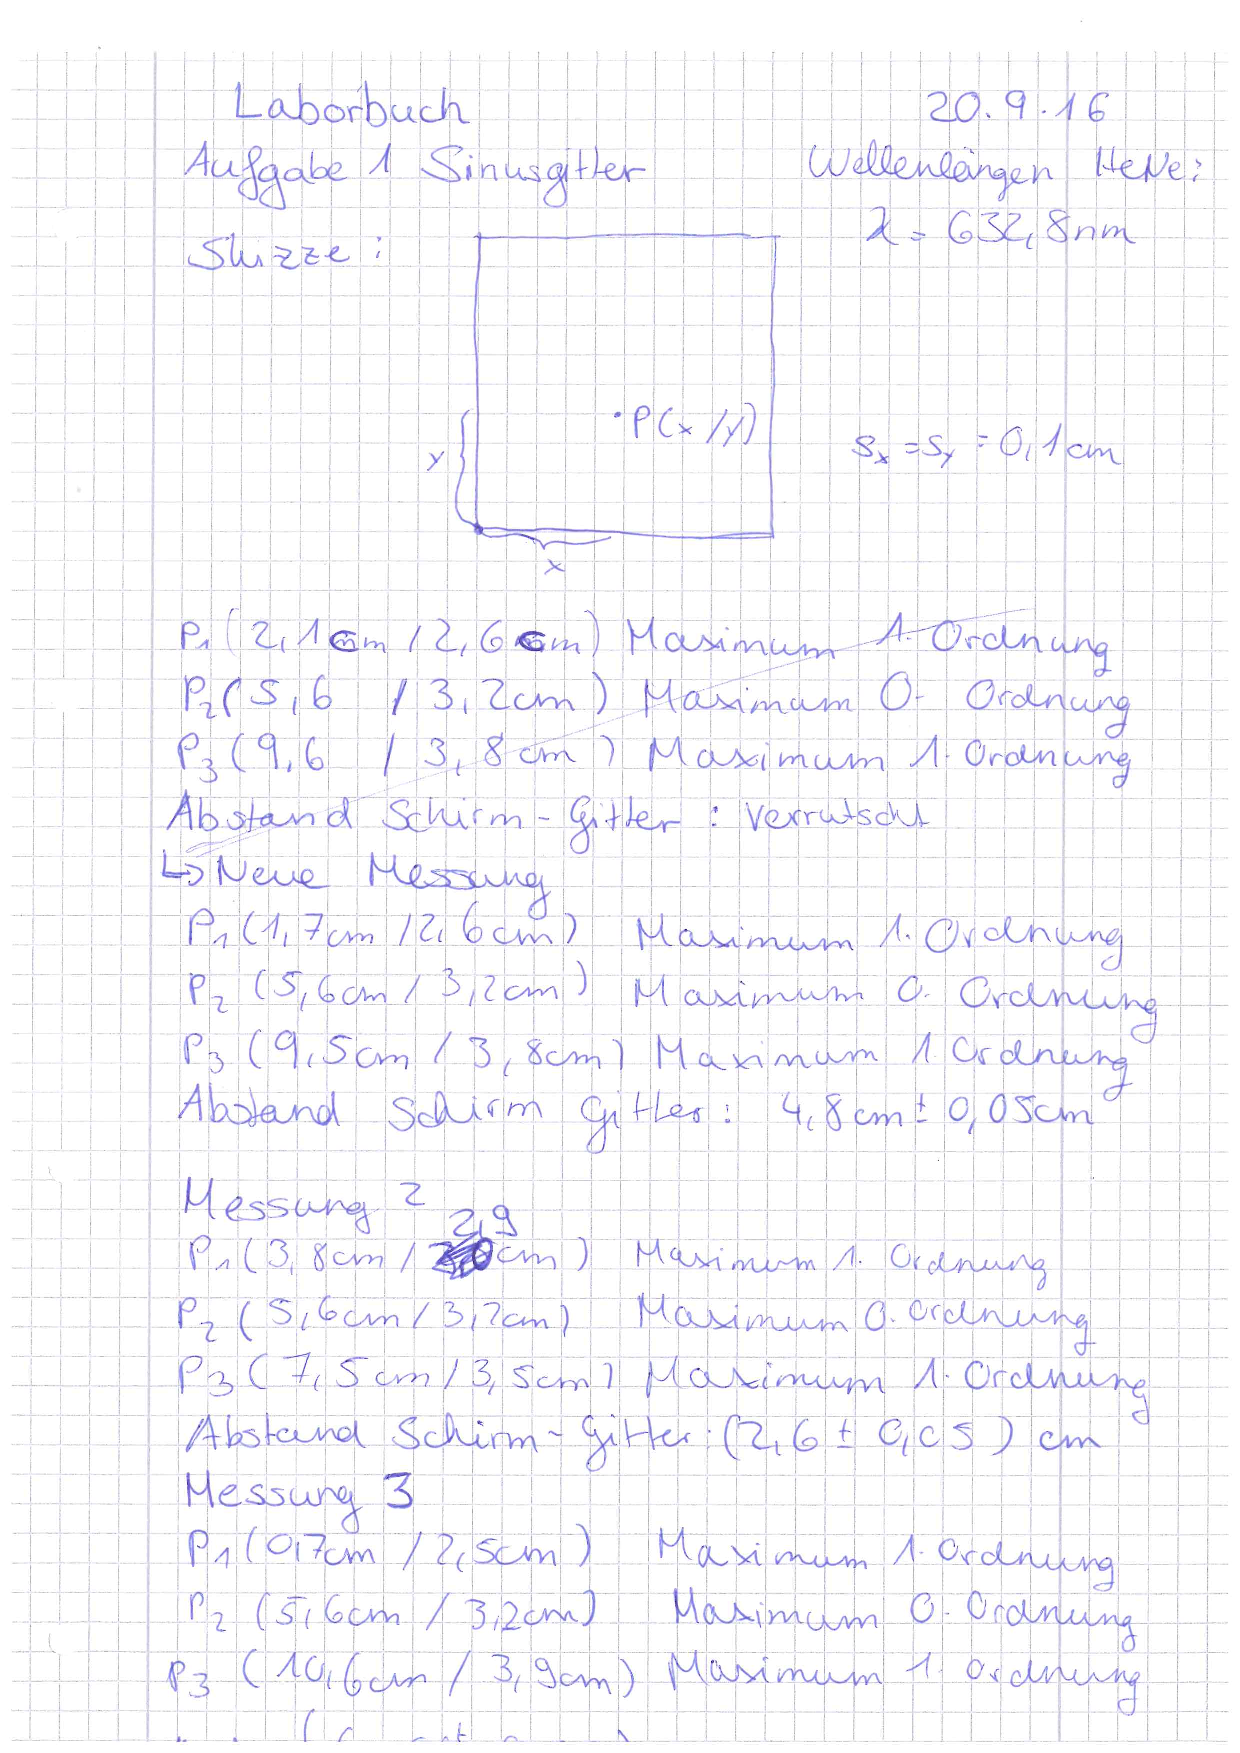
\includegraphics[width=0.9\textwidth]{figures/Laborbuch2.pdf}
\end{minipage}

\begin{minipage}{\textwidth}
\centering
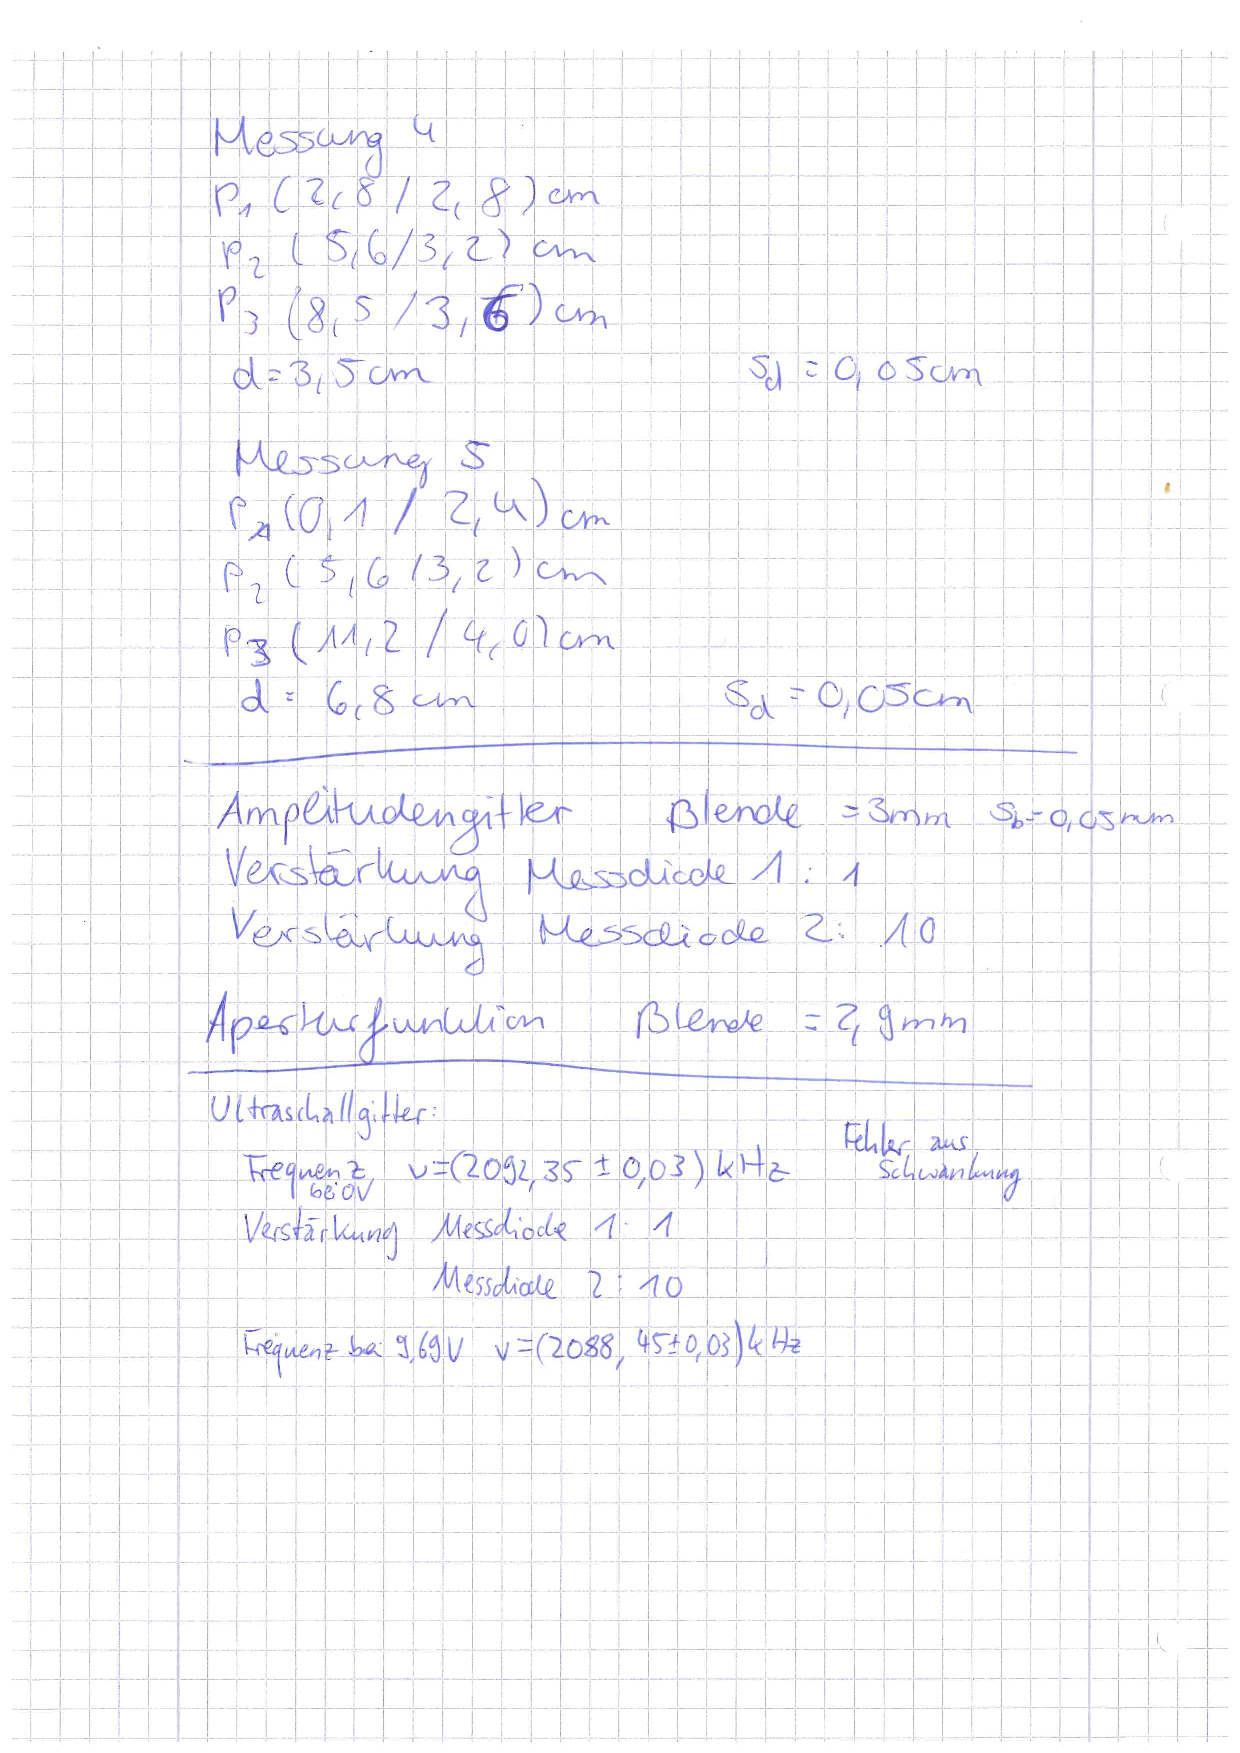
\includegraphics[width=0.9\textwidth]{figures/Laborbuch1.pdf}
\end{minipage}
\newpage
\listoffigures

%Literatur----------------------------------------------------------------------------------------------------------

%\cite{les}
\newpage
\thispagestyle{empty}
\begin{thebibliography}{9}

%\bibitem{staat}
%  Tobijas Kotyk,
%  \emph{Versuche zur Radioaktivität im Physikalischen Fortgeschrittenen Praktikum an der Albert-Ludwigs-Universität Freiburg},
%  Albert-Ludwigs-Universität, Freiburg,
%  2005
  

  
%\bibitem{molmasse}
%  \emph{http://www.convertunits.com/molarmass/<ELEMENTNAME AUF ENGLISCH>}, Stand 28.09.2015
  
\bibitem{staat}
\emph{http://hacol13.physik.uni-freiburg.de/fp/Versuche/FP1/FP1-2-Ultraschall/Staatsex-Ultraschall.pdf}, Stand 23.09.2016

\bibitem{anleitung}
\emph{http://hacol13.physik.uni-freiburg.de/fp/Versuche/FP1/FP1-2-Ultraschall/Anleitung.pdf}, Stand 23.09.2016


\end{thebibliography}

\end{document}